\section{Controller and Observer Design}
\subsection{State and input response}

This system is really complicated and I am unable to find a mathmatical solution to $e^AT$
or $\laplaceinv{(sI-A)^{-1}}$. I even tried to have my computer solve it to no luck
as a result, I am going to plot the response by modeling the system with code required later.
As the system is non-stable it quickly explodes
Zero State Response
\begin{figure}[H]
  \begin{center}
    \makebox[\textwidth]{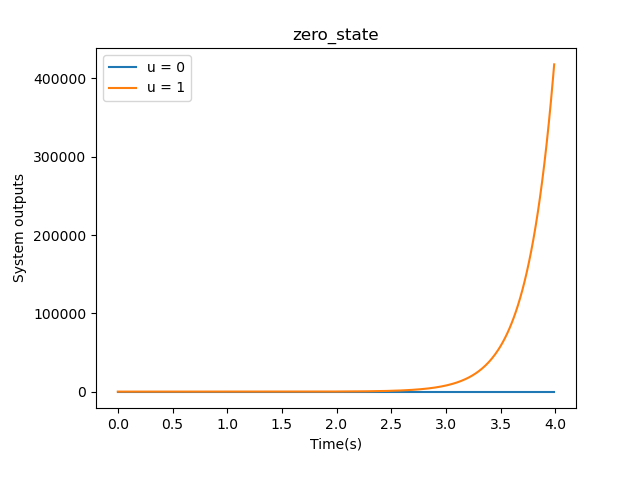
\includegraphics[max width=\textwidth]{../resources/zero_state.png}}
  \end{center}
  \caption{zero state}
  \label{fig:zero_state}
\end{figure}


Zero Input Response
\begin{figure}[H]
  \begin{center}
    \makebox[\textwidth]{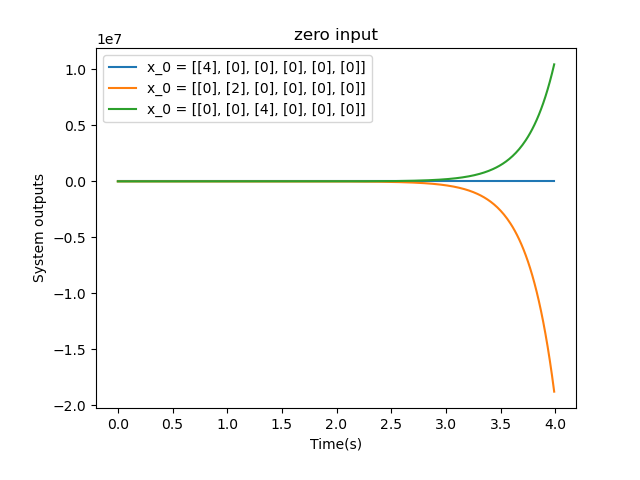
\includegraphics[max width=\textwidth]{../resources/zero input.png}}
  \end{center}
  \caption{Zero input Response}
  \label{fig:zero input}
\end{figure}


As this system is massively unstable, I will only be doing simulation runs with zero input(shown again below)
however, the total state response for a less unstable system is achieved by adding the zero state response
with the zero state response for a given input and state.

Total Response
\begin{figure}[H]
  \begin{center}
    \makebox[\textwidth]{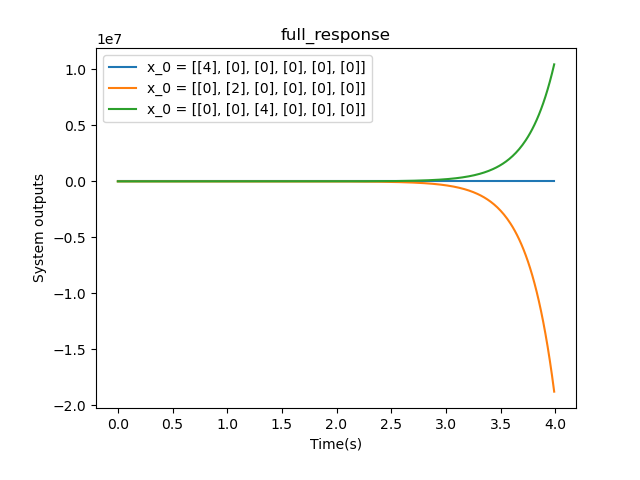
\includegraphics[max width=\textwidth]{../resources/full_response.png}}
  \end{center}
  \caption{Full Response}
  \label{fig:full_response}
\end{figure}
